\documentclass{article}
\usepackage{multicol}
\usepackage{graphicx}
\usepackage[section]{placeins}
\usepackage{hyperref}
\hypersetup{
	colorlinks=true,
	linkcolor=blue,
	filecolor=magenta,      
	urlcolor=cyan,
}
\urlstyle{same}
\usepackage{caption}
\usepackage{listings}





\title{\Huge \bfseries \emph{Assignment 1}}
\author{Vathana Him}
\date{September 12, 2021}

\begin{document}
\maketitle

\begin{multicols}{2}
	
\section{Abstract}
	The purpose of this assignment was to begin the introduction to data preprocessing as a preparation step for machine learning and deep learning. This assignment utilized images from UCI respository as sample datasets that will be used to train a machine learning model. Images that were processed represented three fruits spanish pear, fuji apple, watermelon. 
	
	The data for these images were processed using the OpenCV python library. The main goals for this assignment were to process the data for each respective images into their appropriate feature space and feature vector, analyze thess datasets to see if there were any imbalance, explore if any standardization was needed, and export these data into appropriate .csv format to be used as training datasets for machine learning.  


\section{Setting Up}
The developing environment was installed by going to the anaconda website and downloading anaconda. Then anaconda was launched. Once it was launched, navigate to the environment tab, then the create button was pressed in order to create the new working environment. The enviroment was named as MSIA. Within the environment, python 3.7 was installed. Subsequently, pip was used to install a list of python libraries. These libraries included Opencv, Pandas, Plotly, Matplotlib, and Numpy.


\subsection{Section 1 Figures} 

	\begin{center}
		\captionof{figure}{environment}
		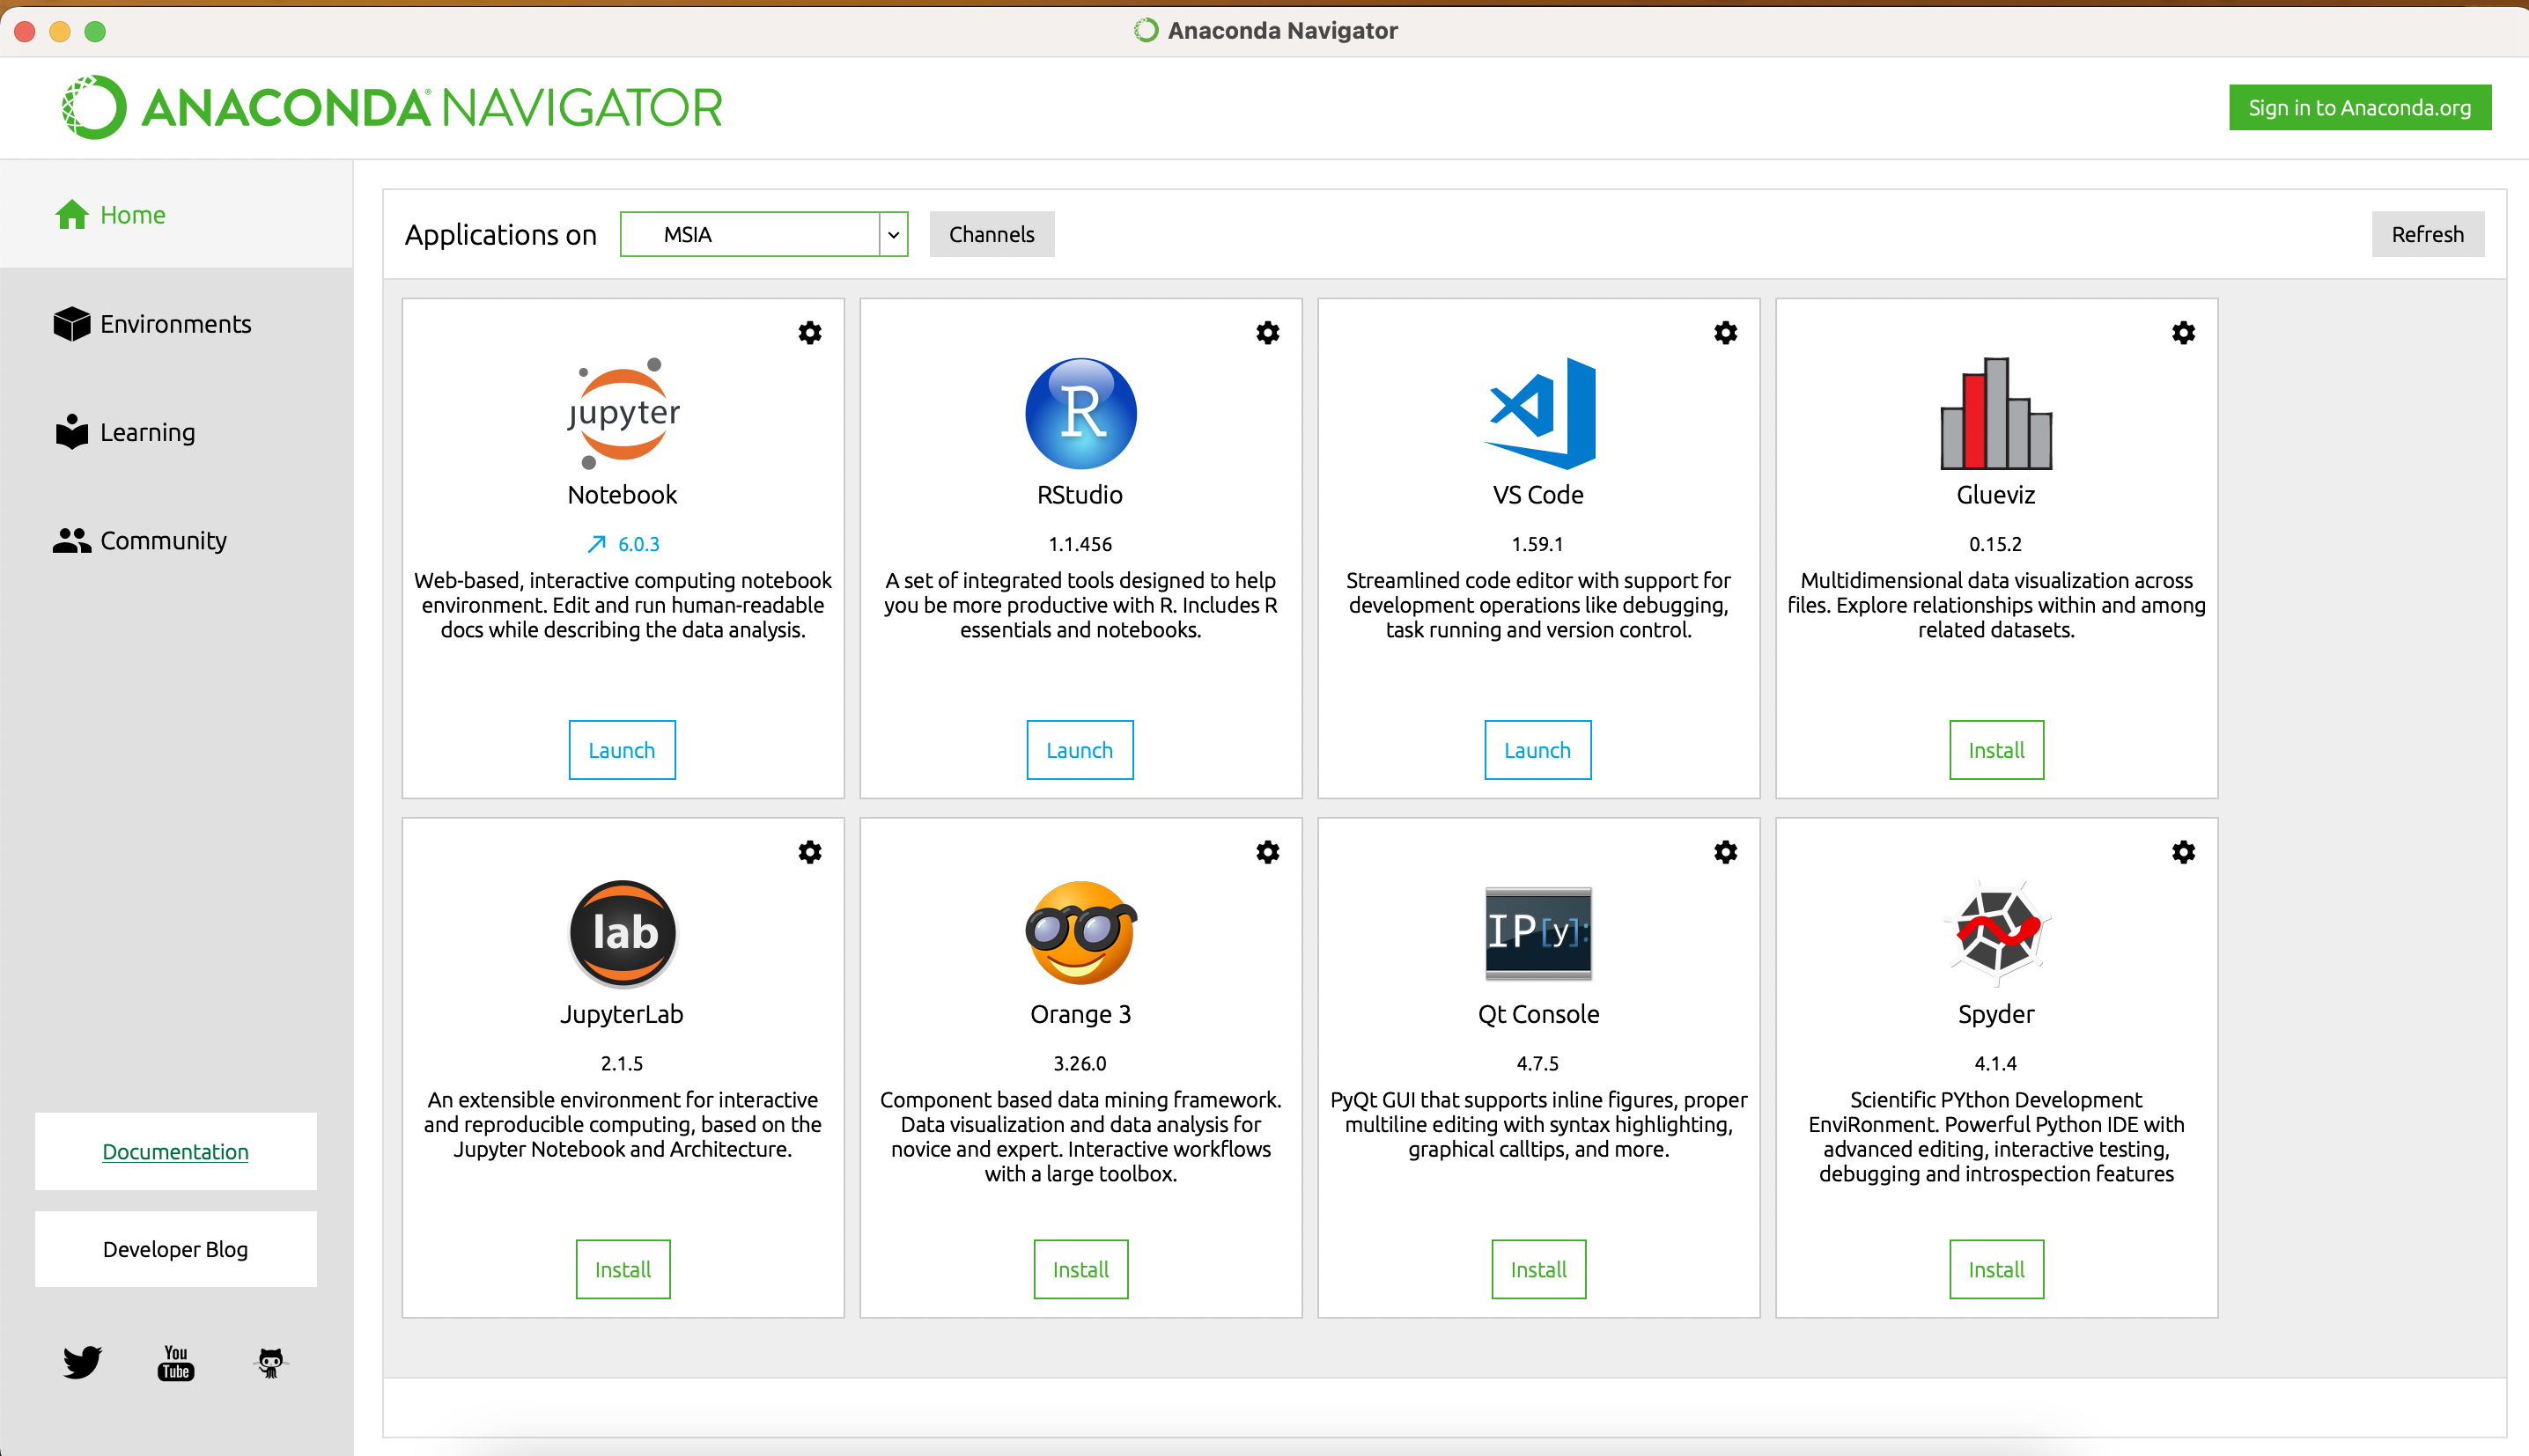
\includegraphics[scale=0.1]{../screenshots/environment.png}
		
	\end{center}

	\captionof{figure}{Pip Command}
	\begin{verbatim}
		Ex.
		pip install pandas
		pip install opencv
	\end{verbatim}
	

	

		
	

\section{Choosen Images}
The choosen images were gathered from the UCI data respository. The link for these images can be found \href{https://www.ic.unicamp.br/~rocha/pub/downloads/}{here} \footnote[1]{https://www.ic.unicamp.br/~rocha/pub/downloads/}. This dataset contains a variety of fruits and vegatables but only three images were choosen for this assignment. These image were spanish pear, fuji apple, and watermelon. Each of these images respresent a fuji apple, spanish pear,
and watermelon respectively. These images were chosen due to the nature of their color as apple was a bright red color, spanish pear was a bright yellow, and watermelon was green. Intuitively, the human eyes was able to distinguish the differences betweent these colors easily. In correlation, computer vision should be able to distinguish the same differences due to its difference in RGB value. Subsequently, these images also have consistent dimensions which makes scaling and resizing of images more consistent.


\subsection{Section 3 Figures} 
\centering
\captionof{figure}{Image Folders}
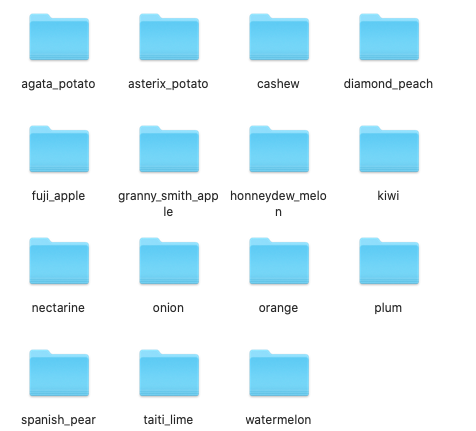
\includegraphics[scale=0.3]{../screenshots/image_folder.png}

\centering
\captionof{figure}{Spanish Pear}
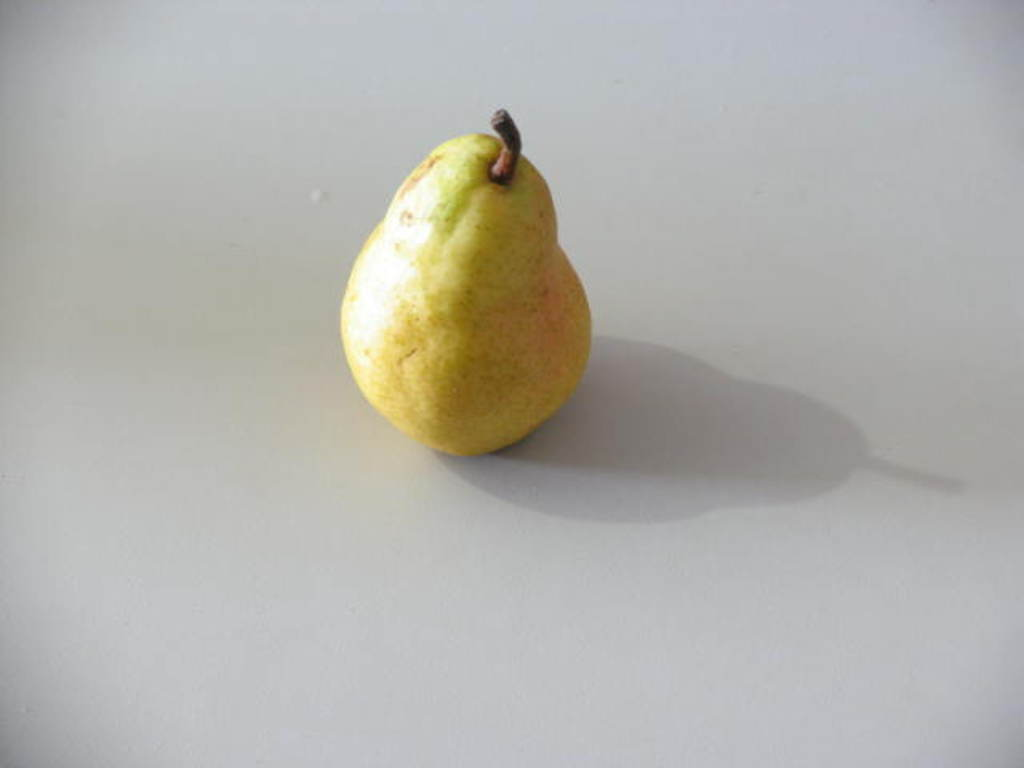
\includegraphics[scale=0.3]{../data/spanish_pear_001.jpg}

\centering
\captionof{figure}{Fuji Apple}
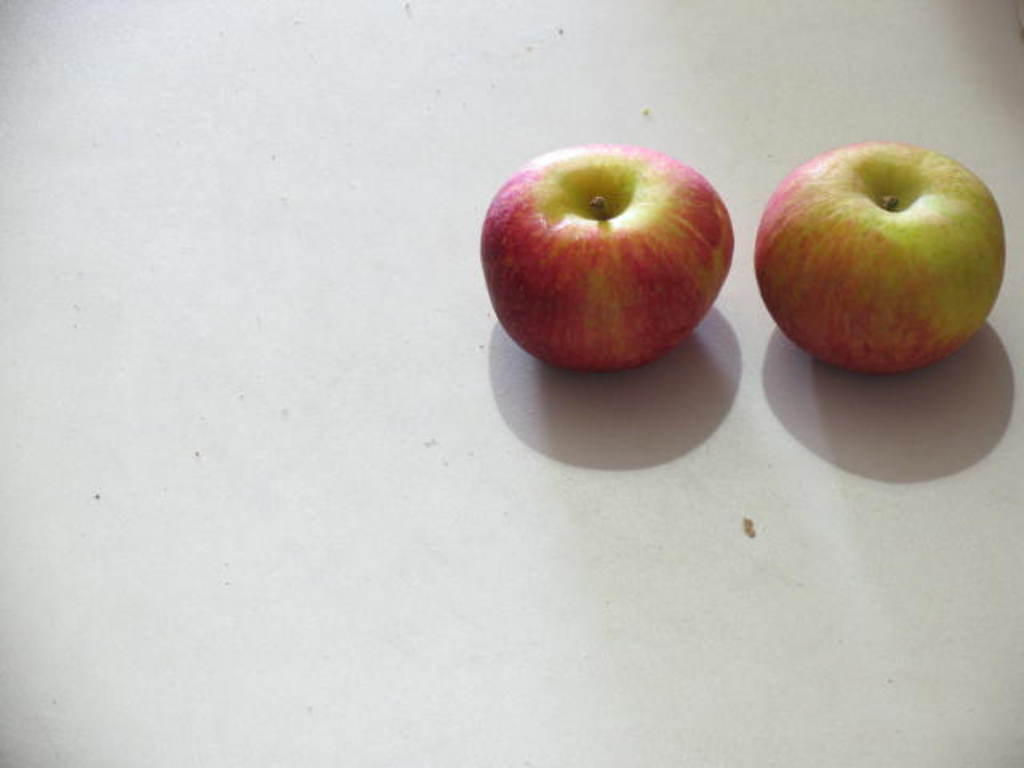
\includegraphics[scale=0.3]{../data/fuji_apple_001.jpg}

\centering
\captionof{figure}{Watermelon}
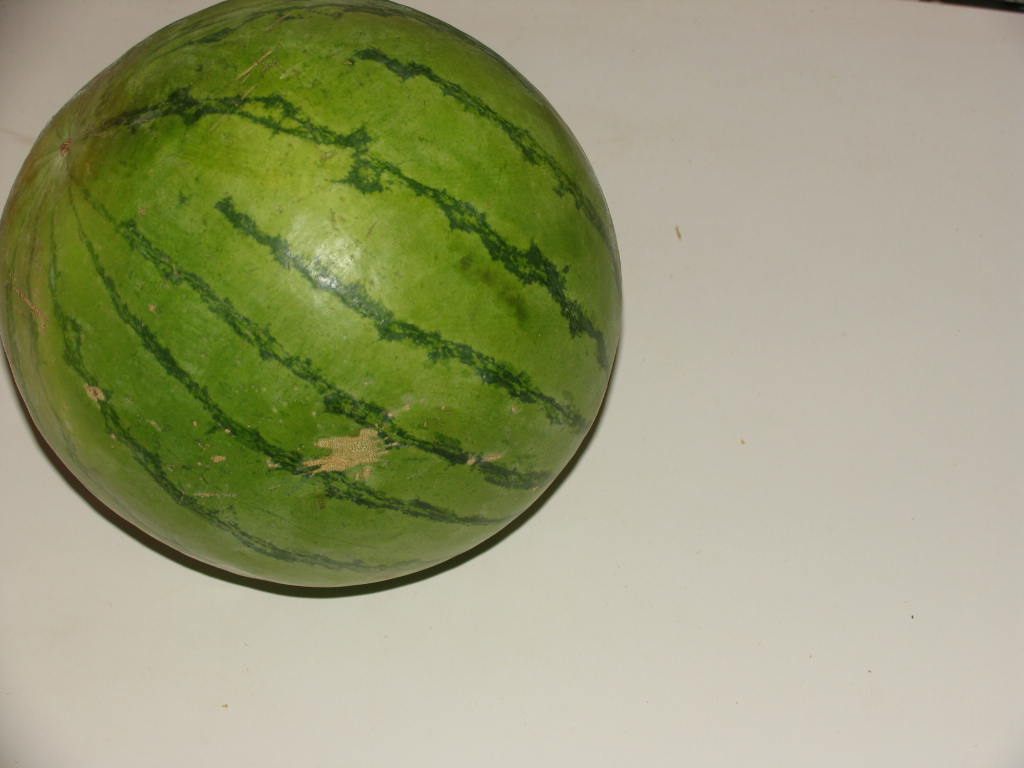
\includegraphics[scale=0.3]{../data/watermelon_001.jpg}

\section{Task 3}

The code to display the three chosen images using python and opencv library is displayed below.

\subsection{Task 3 Results}

\centering
\captionof{figure}{Apple RGB}
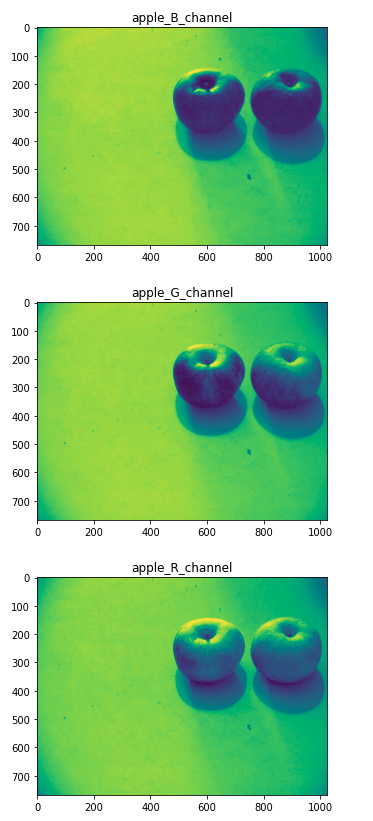
\includegraphics[scale=0.3]{../screenshots/RGB_1.png}

\centering
\captionof{figure}{Pear RGB}
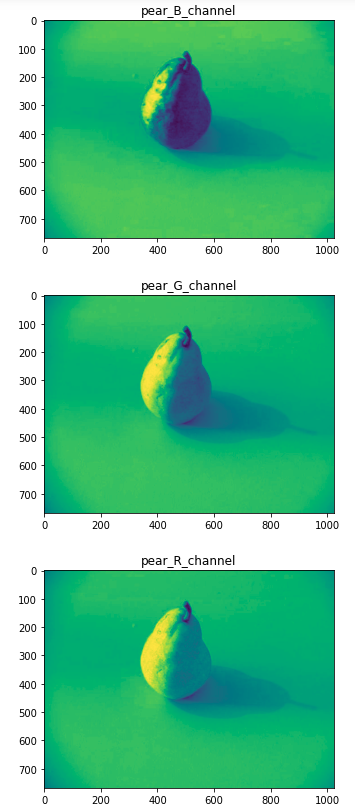
\includegraphics[scale=0.3]{../screenshots/RGB_2.png}

\centering
\captionof{figure}{Watermelon RGB}
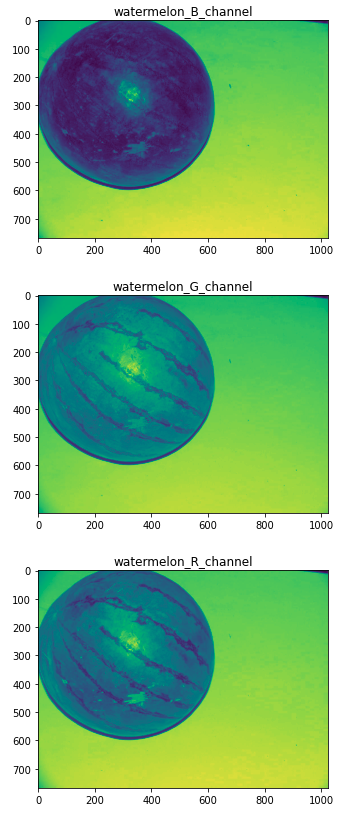
\includegraphics[scale=0.3]{../screenshots/RGB_3.png}

\centering
\captionof{figure}{Gray scale}
\includegraphics[scale=0.3]{../screenshots/gray.png}

\end{multicols}

\subsection{Code}

\centering

\begin{lstlisting}[language=Python]
	import cv2 as cv
	import sys
	import matplotlib.pyplot as plt
	import matplotlib.image as mpimg
	import numpy as np
	import pandas as pd
	img_apple = cv.imread("../data/fuji_apple_001.jpg")
	img_pear = cv.imread("../data/spanish_pear_001.jpg")
	img_watermelon = cv.imread("..data/watermelon_001.jpg")
	
	img_list = [img_apple, img_pear, img_watermelon]
	
	title = ["apple","pear","watermelon"]
	
	color_channel = ["B_channel", "G_channel", "R_channel"]
	
	num = 0
	for i in img_list:
	n = 0
	#split color channel of each image by B, G, R
	for j in cv.split(i):
	plt.figure()
	plt.imshow(j)
	plt.title(title[num]+"_"+color_channel[n])
	n = n+1
	num = num+1
	
	img_list_gray = []
	for i in img_list:
	img = cv.cvtColor(i, cv.COLOR_BGR2GRAY)
	img_list_gray.append(img)
	plt.figure()
	plt.imshow(img, cmap='gray')
	plt.title("dimension {}".format(img.shape))
\end{lstlisting}

\begin{multicols}{2}
	\section{Task 4}
	The grayscale images were then resized and their new dimensions were displayed through matplotlib. There was a function that was used to help create this gray scale image so it can be generalized for future use.	
	\subsection{Task 4 Result}
	\pagebreak
	\centering
	\captionof{figure}{Gray scale}
	\includegraphics[scale=0.25]{../screenshots/gray_resized.png}
\end{multicols}
	\subsection{Code}
	\begin{lstlisting}[language=Python]
	gray_imgresize = []
	
	for i in img_list_gray:
	temp_img = img_resize(344, 256, i)
	gray_imgresize.append(temp_img)
	for i in gray_imgresize:
	plt.figure()
	plt.imshow(i, cmap='gray')
	plt.title("resized gray image dimension {}".format(i.shape))
	\end{lstlisting}

\begin{multicols}{2}
	\section{Task 5}
	The grayscale images were then divided into blocks of 8X8 pixels image. Each feature was then assigned a label respectively to identify them. 
	\subsection{Task 5 Results}
	\centering
	\captionof{figure}{Feature Vector Output}	\includegraphics[scale=0.2]{../screenshots/feature_vector88.png}
	
	\centering
	\captionof{figure}{CSV Output}	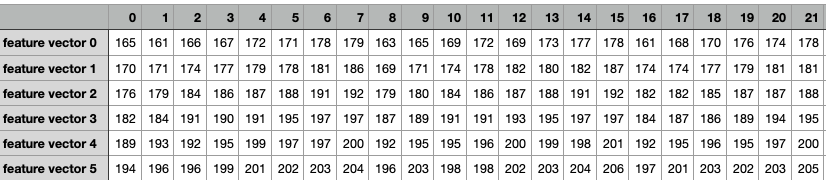
\includegraphics[scale=0.25]{../screenshots/88csv.png}
	\end{multicols}
	
	\pagebreak
	\subsection{Code}
	\begin{lstlisting}[language=Python]
	#convert each image into blocks of 8X8 and store them in a list 
	img_blocks = []
	for i in gray_imgresize:
	img_blocks.append(con_to_img_blocks(i))
	#convert to dictionary of feature value for each image and store all image in a list
	img_feature_list = []
	for i in img_blocks:
	img_feature_list.append(label_feature(i))
	#convert each feature of size 64 vectirs into csv
	for i in range(len(img_feature_list)):
	if (i==0):
	s='img_0'
	elif (i==1):
	s="img_1"
	else:
	s="img_2"
	temp_df = to_dataframe(img_feature_list[i])
	temp_df.to_csv("img_csvs/"+"{}.csv".format(s))
	\end{lstlisting}

\begin{multicols}{2}
	\section{Task 6}
	After being divided into 8X8 pixel blocks, the grayscale images were then divided into sliding block of 8X8 pixels. Each feature was then assigned a label respectively to identify them. Two helper functions were used for this task, sliding blocks feature function which converts an image into sliding image blocks given an image object, and label feature function which create feature labels for each image given a list that contains the array of sliding images.  
	
	\subsection{Task 6 Results}
	\centering
	\captionof{figure}{Feature Vector Output}	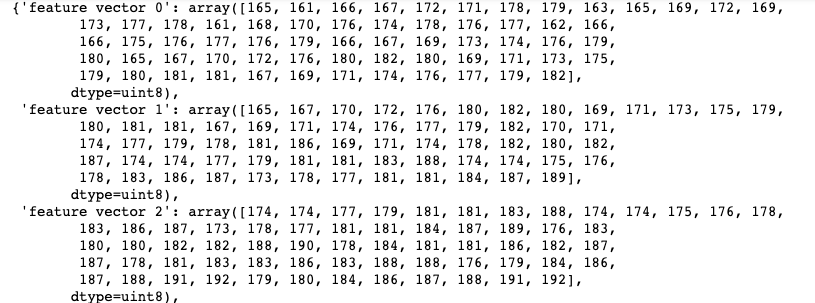
\includegraphics[scale=0.2]{../screenshots/sliding88.png}
	
	\centering
	\captionof{figure}{CSV Output}	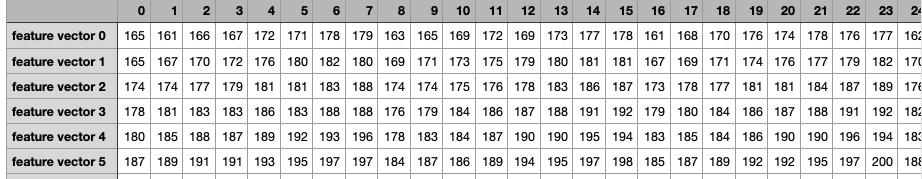
\includegraphics[scale=0.25]{../screenshots/sliding88csv.png}
\end{multicols}

\pagebreak
\subsection{Code}
\begin{lstlisting}[language=Python]
#convert each image into sliding blocks of 8X8 and store them in a list each index of list contains all blocks of each image 
sliding_block_list = [sliding_blocks(i)for i in gray_imgresize]


#convert to dictionary of feature value for each image in sliding block and store all image in a list
sliding_img_feature_list = [label_feature(i) for i in sliding_block_list]
\end{lstlisting}

\begin{multicols}{2}
	\section{Task 7}
		\setlength{\parindent}{10ex}
		The dimension of the gray images were resized 
		to height of 256 and width of 344. 
		The purpose for these choosen dimensions was to keep 
		its aspect ratio. Additionally, the resized height and 
		width must also be divible by eight since this project 
		divided the targeted image into sliding blocks of 8 by 8 
		height and width. The feature vector that was constructed 
		from these images created 3400 feature vectors and each 
		feature vector lies a 8 by 8 pixels who's value lies 
		between 0-255 of the gray image scale. 
		The features of each feature vector was then flatten to 
		64 features for each respective feature vector. 
		
		\setlength{\parindent}{10ex}
		The mean of each feature lies between 189-190 for
		img0 apple, img1 177-178 pear, and img2 148-151 watermelon.
		This data does not need normalization as its mean feature 
		values seem to correlate to the color of each fruit that 
		belong to their respective image. For example, 
		both the color for apple and pear are brighter than 
		that of the color for watermelon, therefore, it should 
		intuitively be true that the mean of each feature in the 
		watermelon image should be lower than that of the brighter 
		colored images. Subsequently, 
		the standard deviation value of each image was 
		normally distributed according to the histogram.
		The mean and variance of img1 and img2 were relatively 
		similar, this indicates that normalization may not be needed. 
		However, normalization may be needed for img0 because its 
		histogram seemed to have a two tail distribution. Its mean and 
		variance values also deviated from the subsequent two images. 
		For img1 and img2 normalization was not 
		needed since their values were normally distributed. 
		This suggests that the data of feature value across 
		all feature vectors was consistent and balanced, 
		thus data transformation may not be needed.  
	
	\subsection{Task 7 Results}
	\centering
	\captionof{figure}{img0 summary stats}	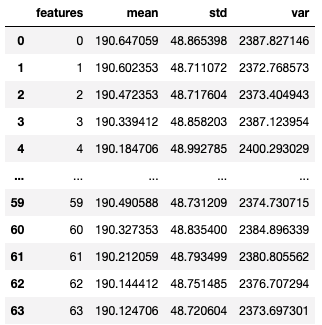
\includegraphics[scale=0.2]{../screenshots/img_0_sum.png}
	
	\centering
	\captionof{figure}{img1 summary stats}	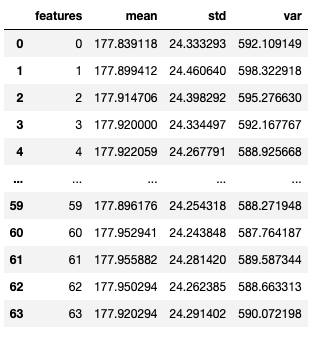
\includegraphics[scale=0.2]{../screenshots/img_1_sum.png}
	
	\centering
	\captionof{figure}{img2 summary stats}	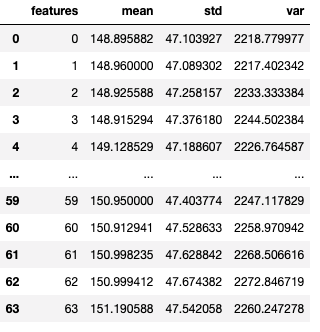
\includegraphics[scale=0.2]{../screenshots/img_2_sum.png}
	
	\centering
	\captionof{figure}{Histogram}	
	\includegraphics[scale=0.3]{../screenshots/histogram.png}
\end{multicols}

\subsection{Code}
\begin{lstlisting}[language=Python]
import matplotlib.pyplot as plt
import plotly.express as px
for i in sliding_block_list:
print(i.shape)
#function to calculate mean, var, std of each feature for each immage, convert it to df for each image respectively and put them in dictionary
def get_stats_img(feature_list):    
stat_dic_img = {}
for i in range(len(feature_list)):
temp_df = to_dataframe(feature_list[i])
temp_df_mean = temp_df.mean().to_frame().reset_index()
temp_df_std = temp_df.std().to_frame().iloc[:,0].values
temp_df_var = temp_df.var().to_frame().iloc[:,0].values
temp_df_mean['std'],temp_df_mean['var'] = [temp_df_std, temp_df_var]
temp_df_mean.columns = ['features', 'mean', 'std', 'var']
stat_dic_img['img_{}'.format(i)] = temp_df_mean
return stat_dic_img
stat_dic_img = get_stats_img(sliding_img_feature_list)
for i in stat_dic_img.keys():
fig = px.histogram(stat_dic_img[i], x=stat_dic_img[i]['mean'], title="mean {}".format(str(i)))
fig.show()
\end{lstlisting}

\begin{multicols}{2}
	\section{Task 8}
	The csvs of image0 and image1 were merged to create a feature space of these images. Similary, a feature space of image0, image1, and image2 was also created by merging their cvs together. Each of these feature spaces were then randomized so it could be used to train a machine learning model for the next assginment. 
	
	\subsection{Task 8 Results}
	\centering
	\captionof{figure}{Merge img01}
	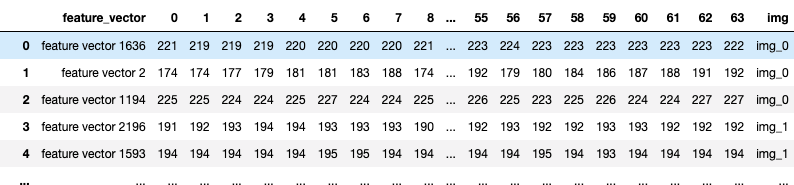
\includegraphics[scale=0.2]{../screenshots/merge01.png}
	
	\centering
	\captionof{figure}{Merge img012}	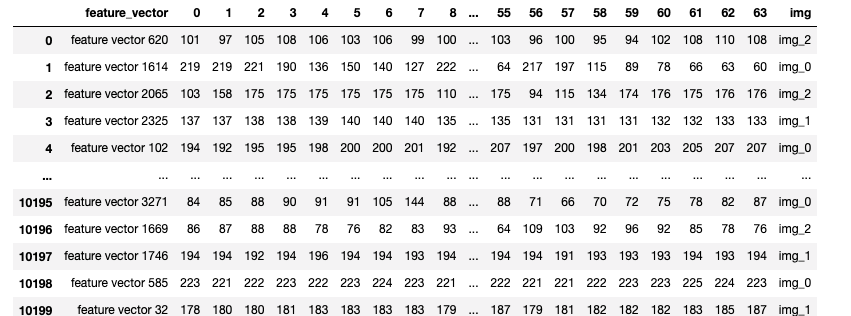
\includegraphics[scale=0.25]{../screenshots/merge012.png}
\end{multicols}

\subsection{Code}
\begin{lstlisting}[language=Python]
	img_0 = pd.read_csv('../data/sliding_img_csvs/sliding_img_0.csv',
	index_col=0)
	img_1 = pd.read_csv('../data/sliding_img_csvs/sliding_img_1.csv', 
	index_col= 0)
	img_2 = pd.read_csv('../data/sliding_img_csvs/sliding_img_2.csv', 
	index_col=0)
	img_0['img'] = "img_0"
	img_1['img'] = "img_1"
	img_2['img'] = "img_2"
	image01 = pd.concat([img_0, img_1]).sample(frac=1)
	image012 = pd.concat([img_0,img_1,img_2]).sample(frac=1)
	image01.to_csv('../data/combined_img_csvs/image01.csv')
	image012.to_csv('../data/combined_img_csvs/image012.csv')
\end{lstlisting}


\begin{multicols}{2}
	\section{Task 9}
	The 2-d feature space plot that showed 
	observations for image0 and image1 indicated 
	that each of their respective feature value was similar. 
	One explaination for this could be that the intensity 
	of their gray color channels were alike. Additionally, 
	there were also some observations that fell out of the 
	mean cluster of the plot. It could be interpreted that 
	these observations represent the color of the different 
	fruits, whereas the observations in the mean of the cluster 
	represent the white spaces of the images. Similarly, 
	when three features of image0 and image1 were selected, 
	there were some observations that fell out the mean cluster, 
	while most observations were within. This relationship supported 
	the earlier analysis that was stated. 
	
	In order to further understand this relationship, 
	a feature space of three class label was plotted. 
	The 2-d feature space plot for the three class labels 
	of their three respective images showed a similar 
	relationship to the two class label plots. 
	The majority of observations within each class 
	lied within the mean cluster as some observations 
	lied outside the mean. Futhermore, this behavior 
	was also observed in the 3-d three features plot 
	where most observations lied within the mean cluster 
	and some observations were outside the mean cluster. 
	This indicated that the majority of the observations 
	between each image had similar color on the gray color 
	scale as the outliers could represent the color on the 
	gray color scale that were indicative to the actual color 
	of each fruits. Thus, further supporting the initial analysis.
	
	Finally, it can be concluded that a feature selection method may be 
	needed in order to eliminate features that are correlated based on evidence displayed in figure 22 and figure 24. 
	
	\subsection{Task 9 Results}
	\centering
	\captionof{figure}{2-D Feature Space img01}
	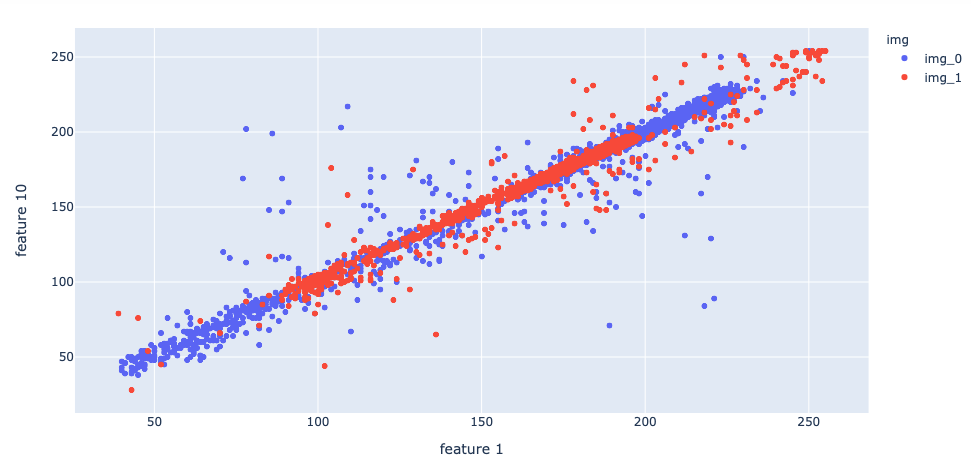
\includegraphics[scale=0.2]{../screenshots/2d01.png}
	
	\centering
	\captionof{figure}{3-D Feature Space img01}	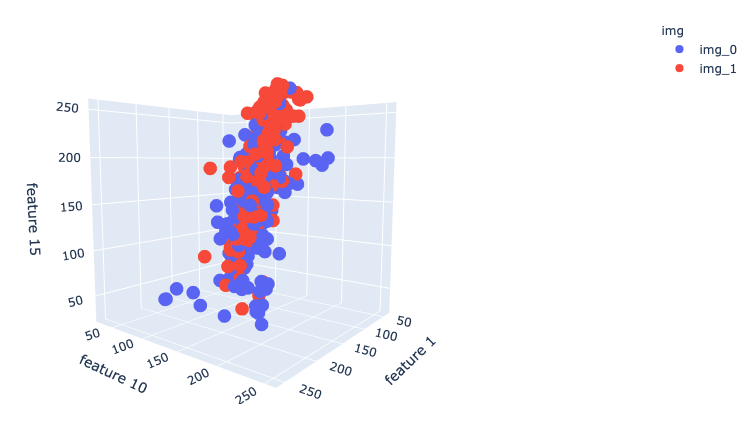
\includegraphics[scale=0.25]{../screenshots/3d01.png}
	
	\centering
	\captionof{figure}{2-D Feature Space img012}
	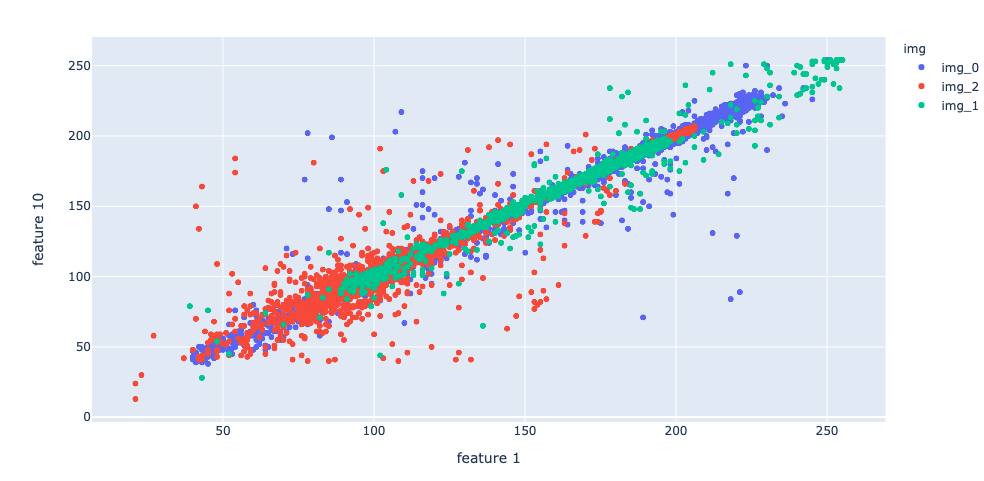
\includegraphics[scale=0.2]{../screenshots/2d012.png}
	
	\centering
	\captionof{figure}{3-D Feature Space img012}	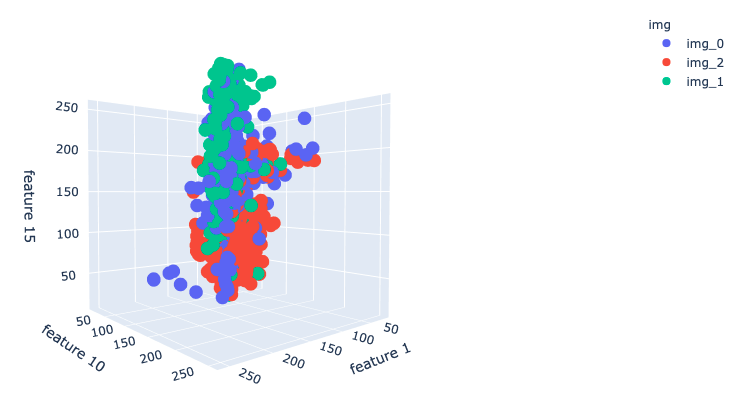
\includegraphics[scale=0.25]{../screenshots/3d012.png}
\end{multicols}

\subsection{Code}
\begin{lstlisting}[language=Python]
fig = px.scatter(df_image01, x='0', y='10', color='img', labels={'10':'feature 10', '0':'feature 1'})
fig.show()
fig = px.scatter_3d(df_image01, x='0', y='10', z='15', color='img', 
labels={'10':'feature 10', '0':'feature 1', '15':'feature 15'})
fig.show()
fig = px.scatter(df_image012, x='0', y='10', color='img', 
labels={'10':'feature 10', '0':'feature 1'})
fig.show()
fig = px.scatter_3d(df_image012, x='0', y='10', z='15', color='img', 
labels={'10':'feature 10', '0':'feature 1', '15':'feature 15'})
fig.show()
\end{lstlisting}

\begin{multicols}{2}
	\section{Task 10}
	Below lists a set of helper functions that can read any number of images from a folder, resize image, convert each image to blocks of 8X8, convert each image to sliding blocks of 8X8, create a dataframe for the feature vectores of each image, and generate the appropriate cvs. These functions was created so that it can be generally used by passing in a python object and it would generate the desired result.
\end{multicols}
\subsection{Code}
\begin{lstlisting}[language=Python]
#helper function

#def get image from given directory
def get_img(path:str):
img_paths = glob.glob(path+"*.jpg")
return img_paths
#read image given a path
def read_img(path:str):
img = cv.imread(path)
return img
#resize image given image object and its width and height
def img_resize(width, height, img):
dim = (width, height)
resized = cv.resize(img, dim, interpolation = cv.INTER_AREA)
return resized

#divide image into 8 by 8 blocks
def con_to_img_blocks(img):
blocks = np.array([img[i:i+8, j:j+8] for j in range(0,344,8) for i in range(0,256,8)]) #iteratre over height and then width
return blocks

#divide image into sliding blocks
def sliding_blocks(img):
step = 5
(w_height, w_width) = (8,8)
slidingblocks = np.array([img[i:i+w_height, j:j+w_width] for j in range(0, img.shape[1]-w_width, step) for i in range(0,img.shape[0]-w_height, step)])
return slidingblocks

#convert each feature of an image into a list of 64 values and add it dictionary with key:feature# and value:list of values of length 64
#return a dictionary of an image with each key as a feature of that image
def label_feature(img):
block_dic = {}
for i in range(len(img)):
block_dic["feature vector {}".format(i)] = img[i].ravel()
return block_dic

#convert a dictionary of an image into pandas dataframe
def to_dataframe(img_dic):
df = pd.DataFrame(img_dic).T
return df

#generate csv given list of dataframe
def to_csv(df_list):
for i in range(len(df_list)):
if (i==0):
s='img_0'
elif (i==1):
s="img_1"
else:
s="img_2"
temp_df = to_dataframe(df_list[i])
temp_df.to_csv("sliding_img_csvs/"+"{}.csv".format(s))
\end{lstlisting}

\begin{multicols}{2}
	\section{Task 11}
	The dimension of original gray images were 256H by 344W. Once divided into sliding blocks, their dimensions were reduced to 8H by 8W of 3400 feature vectors. The pixels representing these blocks were then converted into a one-dimensional array that contains 64 features. Therefore, each feature vectors contain 64 features. These new dimensions were also labeled to represent their images respectively. The conversion of these dimensions to a feature space represented by 64 features would allow machine learning models to distinguish unique features among these images. Classification methods used would allow machine learning modes to understand the differences between the color scale of each pixels within each feature in relation to each feature space and the feature space that belong to their respective image. It would allow machine learning models to understand the differences between each image based on their feature and feature space. Therefore, enabling it to classify future images based on commonality of characteristics from each unique features. 
\end{multicols}


\end{document}